% !TeX root = ellipses.tex

\section{Ellipses in Euclidean geometry}\label{s.geometry}

In this document the proofs of theorems about planetary have freely used analytic geometry and trigonometry. But for many years after the invention of analytic geometry, mathematicians continued to limit themselves to Euclidean geometry, perhaps believing it to be a ``pure'' form of mathematics. Newton, even though he used limits as needed and invented differential calculus (along with Leibntiz), published proofs in Euclidean geometry. Even into the late nineteenth century, students at Cambridge University [ref????] continued to study the original works of Euclid and Newton. In this section, I present proofs in Euclidean geometry (\emph{geometric proofs}) of theorems that appeared before. The presentation is based on the textbook \emph{Conic Sections Treated Geometrically} written by the Cambridge mathematician William H. Besant \cite{besant}.

The section starts with geometric proofs of several theorems on triangles that will be needed below. The next subsection defines ellipses in terms of the geometric concepts of focus and directrix instead of the familiar analytic definition, points which satisfy the following equation for $0<a,b$:
\[
\frac{x^2}{a^2}+\frac{y^2}{b^2}=1\,.
\]



%%%%%%%%%%%%%%%%%%%%%%%%%%%%%%%%%%%%%%%%%%%%%%%%%%%%%%%%%%%%%%%%%%%%%%

\subsection{Theorems on triangles}

%%%%%%%%%%%%%%%%%%%%%%%%%%%%%%%%%%%%%%%%%%%%%%%%%%%%%%%%%%%%%%%%%%%%%%

\subsubsection*{The median of the hypothenuse}

\begin{theorem}
The median to the hypotenuse of a right triangle is equal to half the hypotenuse (Figure~\ref{f.median}). Therefore,
\[
AD \cdot DB = DC^2\,.
\]
\end{theorem}

%%%%%%%%%%%%%%%%%%%%%%%%%%%%%%%%%%%%%%%%%%%%%%%%%%%%%%%%%%%%%%%%%%%%%%

\begin{figure}[b]
\begin{center}
\begin{tikzpicture}

\draw (0,0) coordinate (C) node[below left] {$C$} -- 
  (6,0) coordinate (B) node[right] {$B$} --
  (0,4) coordinate (A) node[above left] {$A$} -- cycle;
\draw (C) rectangle +(6pt,6pt);
\draw (C) -- node[above] {$b$} ($(A)!.5!(B)$)
  coordinate (D) node[above,xshift=2pt] {$D$};
\path (A) -- node[above] {$a$} (D) --
  node[above] {$a$} (B);
\coordinate (E) at ($(C)!.5!(B)$);
\draw[thick,dashed] (D) -- (E) node[below] {$E$};
\draw (E) rectangle +(6pt,6pt);
\path (C) -- node[below] {$c_1$} (E) -- node[below] {$c_2$} (B);
\end{tikzpicture}
\end{center}
\caption{Median to the hypotenuse}\label{f.median}
\end{figure}

\begin{proof}
Drop the perpendicular from $D$ to $BC$ and label the intersection by $E$.

By similar triangles,
\begin{eqn}
\frac{a}{c_2} &=& \frac{a+a}{c_1+c_2}\\[6pt]
c_1&=&c_2\,.
\end{eqn}
Therefore, $\triangle DEC\cong \triangle DEB$ and $DC=DB$.\hqed
\end{proof}

%%%%%%%%%%%%%%%%%%%%%%%%%%%%%%%%%%%%%%%%%%%%%%%%%%%%%%%%%%%%%%%%%%%%%%

\subsubsection*{Adjacent pairs of similar triangles}

I have not encountered the following definition before but it explicitly expresses relation among similar triangles that would have been obvious to geometers.

\begin{definition}
In Figure~\ref{f.adjacent}, $\triangle BAC\sim \triangle EAF$ and $\triangle CAD\sim \triangle FAG$ is an \emph{adjacent pair of similar triangles}.
\end{definition}

\begin{theorem}
For the adjacent pair of similar triangles in Figure~\ref{f.adjacent},
\[
\frac{AB}{AF}=\frac{AD}{AG}\,.
\]
\end{theorem}
\begin{proof} By similar triangles,
\begin{eqn}
\frac{AB}{AF}&=&\frac{AC}{AF}\\[6pt]
\frac{AC}{AF}&=&\frac{AD}{AG}\\[6pt]
\frac{AB}{AF}&=&\frac{AD}{AG}\,.
\end{eqn}\hqed
\end{proof}

Similar ratios hold between other sides of $\triangle BAC$ and $\triangle CAD$ by using an intermediate step with $AC$. We will use the term \emph{by an adjacent pair of similar triangles} and leave it to the reader to make the intermediate step.

\begin{figure}[t]
\begin{center}
\begin{tikzpicture}
\coordinate (X) at (0,0);
\node[left] at (X) {$E$};
\coordinate (S) at (3,0);
\node[right,xshift=4pt] at (S) {$G$};
\draw[name path=directrix] ($(X)+(0,2.4)$) coordinate (K) -- 
  ($(X)+(0,-2)$) coordinate (E);
\node[left] at (E) {$A$};
\node[left] at (K) {$B$};

% Eccentricity 1/2
\coordinate (A) at (2,0);
\node[above left] at (A) {$F$};

\path[name path=EA] (E) -- ($(E)!2.3!(A)$);

\path[name path=ES] (E) -- ($(E)!2.3!(S)$);

\path[name path=SP] (S) -- +(60:3);
\path [name intersections = {of = EA and SP, by = {P} }];
\node[above] at (P) {$C$};

\path[name path=PK] (P) -- +(180:4.5);
\path [name intersections = {of = PK and directrix, by = {K} }];
\path[name path=PL] (K) -- ($(K)!1.7!(P)$);
\path [name intersections = {of = PL and ES, by = {L} }];
\node[above] at (L) {$D$};

\draw[red,thick] (P) -- (L) -- (E) -- cycle;
\draw[blue,thick] ($(E)+(0,3pt)$) -- (K) -- ($(P)+(-3pt,0)$) -- cycle;
\draw[blue,thick] (X) -- ($(A)+(-3pt,0)$);
\draw[red,thick] (A) -- (S);
\end{tikzpicture}
\end{center}
\caption{Adjacent pairs of similar triangles}\label{f.adjacent}
\end{figure}

%%%%%%%%%%%%%%%%%%%%%%%%%%%%%%%%%%%%%%%%%%%%%%%%%%%%%%%%%%%%%%%%%%%%%%

\subsubsection*{The angle bisector theorems}

The angle bisector theorems, which are not well-known to students today, were used extensively in the study of conic systems, often implicitly.
\begin{theorem}[Interior angle bisector theorem]
\label{thm.interior-angle-bisector}
In $\triangle ABC$ let $D$ be a point on $BC$ (Figure~\ref{f.interior-angle-bisector}). Then $AD$ bisects $\angle CAB$ if and only if
\[
\frac {BD}{CD}=\frac {AB}{AC}\,.
\]
\end{theorem}
%%%%%%%%%%%%%%%%%%%%%%%%%%%%%%%%%%%%%%%%%%%%%%%%%%%%%%%%%%%%%%%%%%%%%%

\begin{figure}[b]
\begin{center}
\begin{tikzpicture}[scale=.9]

% Draw base and paths of two lines at known angles
\draw (0,0) coordinate (b) node[left] {$B$} -- 
  (8,0) coordinate (c) node[right] {$C$};
\path[name path=ba] (b) -- +(30:8);
\path[name path=ca] (c) -- +(140:6);

% Get their intersection and draw lines between vertices
\path[name intersections={of=ba and ca,by=a}];
\node[above] at (a) {$A$};
\draw[name path=bc] (b) -- (c);
\draw (b) -- (a) -- (c);

% Draw bisector
\path[name path=bisector] (a) -- +(-95:5.5);
\path[name intersections={of= bc and bisector,by=d}];
\node[below left] at (d) {$D$};

\path[name path=ce] (c) -- +(210:5);
\path[name intersections={of= bisector and ce,by=e}];
\node[left] at (e) {$E$};
\draw[thick,dashed] (c) -- (e);
\draw (a) -- (e);

% Label angles
\node[below left,xshift=-2pt,yshift=-8pt] at (a) {$\alpha$};
\node[below right,xshift=0pt,yshift=-8pt] at (a) {$\alpha$};
\node[above right,xshift=0pt,yshift=6pt] at (e) {$\alpha$};
\node[above left,xshift=0pt,yshift=0pt] at (d) {$\beta$};
\node[below right,xshift=0pt,yshift=0pt] at (d) {$\beta$};

\end{tikzpicture}
\end{center}
\caption{The interior angle bisector theorem}
\label{f.interior-angle-bisector}
\end{figure}

%%%%%%%%%%%%%%%%%%%%%%%%%%%%%%%%%%%%%%%%%%%%%%%%%%%%%%%%%%%%%%%%%%%%%%

\begin{proof}
Construct a line through $C$ parallel to $AB$ and let its intersection with $AD$ be $E$. By alternate interior angles, $\angle BAD=\angle AEC=$ and by vertical angles $\angle BDA=\angle CDE$. Therefore, $\triangle ABD\sim \triangle EDC$ so
\[
\frac{BD}{CD}=\frac{AB}{CE}\,.
\]
$\triangle ECA$ is isoceles so $CE=AC$ and
\[
\frac{BD}{CD}=\frac{AB}{AC}\,.
\]
To prove the converse just ``run'' the proof backwards.
\hqed
\end{proof}

%%%%%%%%%%%%%%%%%%%%%%%%%%%%%%%%%%%%%%%%%%%%%%%%%%%%%%%%%%%%%%%%%%%%%%

\begin{theorem}[Exterior angle bisector theorem]
\label{thm.exterior-angle-bisector}
In $\triangle ABC$ let $D$ be a point on the extension of $CB$ outside the triangle (Figure~\ref{f.exterior-angle-bisector}). Then $AD$ bisects the supplementary angle of $\angle BAC$ if and only if
\[
\frac {BD}{CD}=\frac {AB}{AC}\,.
\]
\end{theorem}

%%%%%%%%%%%%%%%%%%%%%%%%%%%%%%%%%%%%%%%%%%%%%%%%%%%%%%%%%%%%%%%%%%%%%%

\begin{figure}
\begin{center}
\begin{tikzpicture}[scale=1.2]

% Draw base and paths of two lines at known angles
\path (0,0) coordinate (b) node[below] {$B$} -- 
  (8,0) coordinate (c) node[below] {$C$};
\path[name path=ba] (b) -- +(50:3);
\path[name path=ca] (c) -- +(170:7.5);

% Get their intersection and draw lines between vertices
\path[name intersections={of=ba and ca,by=a}];
\node[above] at (a) {$A$};
\path[name path=bc] (c) -- ($(c)!1.5!(b)$);
\draw[red,thick] (b) -- (a) -- (c) -- cycle;
\path (c) -- ($(c)!1.4!(a)$) coordinate (f);
\draw (a) -- (f) node[above] {$F$};
% Draw bisector
\path[name path=bisector] (a) -- +(200:5.5);
\path[name intersections={of= bc and bisector,by=d}];
\node[below] at (d) {$D$};
\draw[thick,red,dashed] (b) -- (d);
\draw[thick,blue] (a) -- (d);

\path[name path=be] (b) -- +(20:4);
\path[name intersections={of= be and ca,by=e}];
\node[above] at (e) {$E$};
\draw[thick,dashed] (b) -- (e);

% Label angles
\node[left,xshift=-12pt,yshift=-2pt] at (a) {$\alpha$};
\node[below left,xshift=-10pt,yshift=-6pt] at (a) {$\alpha$};
\node[above right,xshift=10pt,yshift=6pt] at (b) {$\alpha$};
\node[left,xshift=-10pt,yshift=-2pt] at (e) {$\alpha$};

\end{tikzpicture}
\end{center}
\caption{The exterior angle bisector theorem}
\label{f.exterior-angle-bisector}
\end{figure}

%%%%%%%%%%%%%%%%%%%%%%%%%%%%%%%%%%%%%%%%%%%%%%%%%%%%%%%%%%%%%%%%%%%%%%

\begin{proof}
Construct a line through $B$ parallel to $AD$ and let its intersection with $AC$ be $E$. By alternate interior angles $\angle BAD=\angle ABE$ and by corresponding angles $\angle FAD=\angle AEB$. Therefore, $\triangle BCE\sim \triangle DCA$ so
\[
\frac{BD}{CD}=\frac{AE}{AC}\,.
\]
$\triangle BAE$ is isoceles so $AE=AB$ and
\[
\frac{BD}{CD}=\frac{AB}{AC}\,.
\]
To prove the converse just ``run'' the proof backwards.
\hqed
\end{proof}

\begin{center}
\fbox{\parbox{.8\textwidth}{The exterior angle bisector theoren confusing to understand in a proof, because it can be hard to identify the components of a diagram. The following color-coding is used below: triangle is red, the extension of one side is dashed red and the bisector is blue.}}
\end{center}


%%%%%%%%%%%%%%%%%%%%%%%%%%%%%%%%%%%%%%%%%%%%%%%%%%%%%%%%%%%%%%%%%%%%%%

\subsection{The definition of an ellipse using the focus and the directrix}

\begin{definition}
Let $d$ be a line (the \emph{directrix}) and $S$ be a point (the \emph{focus}) not on the directrix. Let $0<e<1$ be a number (the \emph{eccentricity}). An \emph{ellipse} is the geometric locus of points such that the ratio of its distance to the focus to its distance to the directrix is $e$.
\end{definition}

All the conic sections (parabolas, ellipses and hyperbolas) are defined the same way and are distinguished by their eccentricity. You might be familiar with the definition of the parabola where $e=1$ (Figure~\ref{f.parabola}).

\begin{figure}[b]
\begin{center}
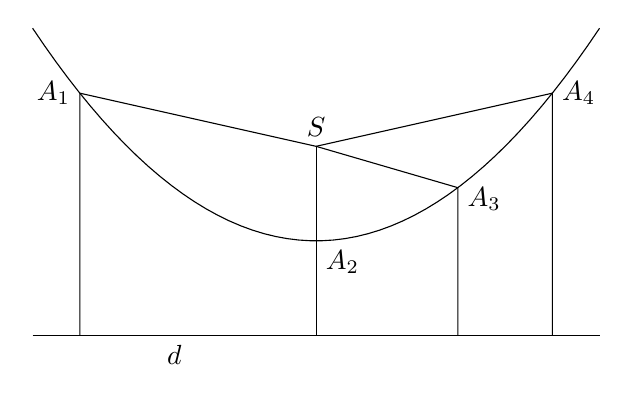
\begin{tikzpicture}[scale=.6]
\draw (-6,-2) -- node[below,near start] {$d$} (6,-2);
\draw[domain=-6:6,samples=50] plot (\x,{\x*\x/8});
\coordinate (F) at (0,2);
\vertexsm{F};
\node[above] at (F) {$S$};
\coordinate (vertex) at (0,0);
\node[below right] at (vertex) {$A_2$};
\coordinate (FP) at (-5,-2);
\coordinate (F2) at (3,1.125);
\node[right,yshift=-4pt] at (F2) {$A_3$};
\coordinate (F3) at (5,3.125);
\node[right] at (F3) {$A_4$};
\coordinate (F4) at (-5,3.125);
\node[left] at (F4) {$A_1$};
\draw (F) -- (0,-2);
\draw (F) -- (F2) -- (3,-2);
\draw (F) -- (F3) -- (5,-2);
\draw (F) -- (F4) -- (FP);
\end{tikzpicture}
\end{center}
\caption{A parabola defined by the focus and the directrix}\label{f.parabola}
\end{figure}

\begin{definition}
Let $X$ be the intersection of the perpendicular to the directrix from $S$. $A$ on $SX$ is a \emph{vertex} of the ellipse if $SA/AX=e$ (in Figure~\ref{f.def-ellipse}, $e=1/2$).
\end{definition}

%%%%%%%%%%%%%%%%%%%%%%%%%%%%%%%%%%%%%%%%%%%%%%%%%%%%%%%%%%

\begin{figure}
\begin{center}
\begin{tikzpicture}

% Construct the directrix, the focus and the perpendicular
\coordinate (X) at (0,0);
\node[left] at (X) {$X$};
\coordinate (S) at (3,0);
\node[below] at (S) {$S$};
\draw[name path=directrix] ($(X)+(0,2)$) --
  node[left,near start] {$d$} ($(X)+(0,-2)$);
\draw (S) -- node[above left] {$1$} (A) -- node[above] {$2$} (X);

% Locate the vertex with eccentricity 1/2
\coordinate (A) at (2,0);
\node[below] at (A) {$A$};

\vertexsm{X};
\vertexsm{S};
\vertexsm{A};
\end{tikzpicture}
\end{center}
\caption{The elements of the definition of an ellipse}\label{f.def-ellipse}
\end{figure}

%%%%%%%%%%%%%%%%%%%%%%%%%%%%%%%%%%%%%%%%%%%%%%%%%%%%%%%%%%

\subsubsection*{Constructing the vertices}

Given $e=SA/AX$ we can locate $A$ as follows:
\begin{eqn}
SA+AX&=&SX\\[4pt]
SA&=&SX\cdot \frac{e}{1+e}\\[4pt]
AX&=&SX\cdot \frac{1}{1+e}\,.
\end{eqn}
Similarly, there is a second vertex $A'$ where
\begin{eqn}
A'X-SA'&=&SX\\[4pt]
SA'&=&SX\cdot \frac{1}{1-e}\\[4pt]
A'X&=&SX\cdot \frac{2-e}{1-e}\,.
\end{eqn}
For example, if $SX=3,e=1/3$ then $SA=1,AX=2$, and $SA'=9/2,A'X=15/2$.

%%%%%%%%%%%%%%%%%%%%%%%%%%%%%%%%%%%%%%%%%%%%%%%%%%%%%%%%%%

\subsubsection*{Constructing points on an ellipse}

Select an \emph{arbitrary} point $E$ on the directrix and construct lines from $E$ through $A$ and $S$. The line through $S$ will make an angle $\alpha$ with $SX$. Construct a line from $S$ at the \emph{same angle} $\alpha$ from $ES$ and let its intersection with $EA$ be $P$. Construct the perpendicular from $P$ to the directrix and let $K$ be its intersection with the directrix. Let $L$ be the intersection of $KP$ with $ES$ (Figure~\ref{f.construct}). 

%%%%%%%%%%%%%%%%%%%%%%%%%%%%%%%%%%%%%%%%%%%%%%%%%%%%%%%%%%

\begin{figure}[t]
\begin{center}
\begin{tikzpicture}[scale=1.2]
\coordinate (X) at (0,0);
\node[left] at (X) {$X$};
\coordinate (S) at (3,0);
\node[below right] at (S) {$S$};
\draw[name path=directrix] ($(X)+(0,2.2)$) -- node[left,near start] {$d$} ($(X)+(0,-2.2)$);

\draw (X) -| ($(X)!2.4!(S)$) node[right] {$N$};

% Eccentricity 1/2
\coordinate (A) at (2,0);
\node[above left] at (A) {$A$};

% Find a convenient E
\path[name path=findE] (S) -- +(210:4);
\path [name intersections = {of = findE and directrix, by = {E} }];

%\coordinate (E) at (0,-1.5);
\node[left] at (E) {$E$};
\draw[name path=EA] (E) -- ($(E)!2.3!(A)$);

\draw[name path=ES] (E) -- ($(E)!2.3!(S)$);

\draw[name path=SP] (S) -- +(60:3) coordinate (Q);
\path [name intersections = {of = EA and SP, by = {P} }];
\node[above left] at (P) {$P$};
\node[left] at (Q) {$Q$};

\path[name path=PK] (P) -- +(180:4.5);
\path [name intersections = {of = PK and directrix, by = {K} }];
\node[left] at (K) {$K$};
\draw[name path=PL] (K) -- ($(K)!2!(P)$);
\path [name intersections = {of = PL and ES, by = {L} }];
\node[above] at (L) {$L$};

\node[right,xshift=12pt,yshift=5pt] at (S) {$\alpha$};
\node[above right,xshift=6pt,yshift=6pt] at (S) {$\alpha$};
\node[below left,xshift=-12pt,yshift=2pt] at (L) {$\alpha$};

\draw[red,very thick] (P) -- (L) -- (E) -- cycle;
\draw[blue,very thick] (E) -- (K) -- ($(P)+(-3pt,0)$) -- ($(E)+(0,3pt)$);

\path (S) -- node[left] {$b$} (P) -- node[above] {$b$} (L);
\end{tikzpicture}
\end{center}
\caption{Constructing points on the ellipse}\label{f.construct}
\end{figure}

%%%%%%%%%%%%%%%%%%%%%%%%%%%%%%%%%%%%%%%%%%%%%%%%%%%%%%%%%%

\begin{theorem}\label{thm.point-on-an-ellipse}
The point $P$ is on the ellipse.
\end{theorem}
\begin{proof}
$\angle PLS = \angle LSN$ by alternate interior angles, so $\triangle LPS$ is isoceles and $PL=SP$. Since $PK\parallel SX$, $\triangle XEA\sim \triangle KEP$ and $\triangle AES\sim \triangle PEL$ are adjacent pairs of similar triangles, so
\begin{eqn}
%\frac{PL}{AS}&=&\frac{PK}{AX}\\
\frac{PL}{PK}&=&\frac{SA}{AX}\\
\frac{PS}{PK}&=&\frac{SA}{AX}= e\,.
\end{eqn}
Therefore, $P$ is on the ellipse since the ratio of its distance from the focus to its distance from directrix is equal to $e$.\hqed
\end{proof}

%%%%%%%%%%%%%%%%%%%%%%%%%%%%%%%%%%%%%%%%%%%%%%%%%%%%%%%%%%

\begin{figure}[b]
\begin{center}
\begin{tikzpicture}[scale=1.2]
\coordinate (X) at (0,0);
\node[left] at (X) {$X$};
\coordinate (S) at (3,0);
\node[below right] at (S) {$S$};
\draw[name path=directrix] ($(X)+(0,2.2)$) -- ($(X)+(0,-2.2)$);

\draw (X) -| ($(X)!2.4!(S)$) node[right] {$N$};

\draw[name path=SP] (S) -- +(60:2) coordinate (P);
\node[above left] at (P) {$P$};

% Find a convenient E
\path[name path=findE] (S) -- +(210:4);
\path [name intersections = {of = findE and directrix, by = {E} }];
\node[left] at (E) {$F$};

\path[name path=PK] (P) -- +(180:4.5);
\path [name intersections = {of = PK and directrix, by = {K} }];
\node[left] at (K) {$K$};
\path[name path=PL] (K) -- ($(K)!2!(P)$);
\draw[name path=ES] (E) -- ($(E)!2!(S)$);
\path [name intersections = {of = PL and ES, by = {L} }];
\node[above] at (L) {$P'$};

\draw[blue,thick] (K) -- (S);

\draw[red,thick] (L) -- (S) -- (P) -- cycle;

\draw[thick] ($(S)+(60:10pt)$)
  arc[start angle=60,end angle=210,radius=10pt];
%\draw[thick] ($(S)+(150:10pt)$)
%  arc[start angle=150,end angle=210,radius=10pt];
\node[above,xshift=-4pt,yshift=8pt] at (S) {$\beta$};
\node[left,xshift=-14pt,yshift=4pt] at (S) {$\beta$};

\draw[thick,dashed,red] (K) -- (P);
\end{tikzpicture}
\end{center}
\caption{Constructing another vertex on $KP$}\label{f.other-vertex}
\end{figure}

%%%%%%%%%%%%%%%%%%%%%%%%%%%%%%%%%%%%%%%%%%%%%%%%%%%%%%%%%%

We now construct another point on $KP$. Construct a line from $F$ on the directrix through $P$ such that $\angle FSK = \angle KSP$ (Figure~\ref{f.other-vertex}).
\begin{theorem}
$P'$, the intersection of $FS$ with $KP$, is on the ellipse.
\end{theorem}

\enlargethispage{\baselineskip}
\begin{proof}
Since $KS$ bisects $\angle PSF$, by the exterior angle bisector theorem 
\begin{eqn}
\frac{SP'}{SP}&=&\frac{P'K}{PK}\\
\frac{SP'}{P'K}&=&\frac{SP}{PK}=e\,,
\end{eqn}
since $P$ is on the ellipse.\hqed
\end{proof}

%%%%%%%%%%%%%%%%%%%%%%%%%%%%%%%%%%%%%%%%%%%%%%%%%%%%%%%%%%

\subsection{Constructing a focal chord}

\begin{definition}
Let $P,P'$ be points on an ellipse. $PP'$ is a \emph{focal chord} of the ellipse if $PP'$ is a chord through a focus (Figure~\ref{f.focal-chord}).
\end{definition}

%%%%%%%%%%%%%%%%%%%%%%%%%%%%%%%%%%%%%%%%%%%%%%%%%%%%%%%%%%

\begin{figure}
\begin{center}
\begin{tikzpicture}[scale=1.4]
\coordinate (X) at (0,0);
\node[left] at (X) {$X$};
\coordinate (S) at (3,0);
\node[below right] at (S) {$S$};
\path[name path=directrix] ($(X)+(0,2.2)$) -- ($(X)+(0,-2.2)$);

\draw (X) -| ($(X)!2.4!(S)$) node[right] {$N$};

% Eccentricity 1/2
\coordinate (A) at (2,0);
\node[above left] at (A) {$A$};

% Find a convenient E
\path[name path=findE] (S) -- +(210:4);
\path [name intersections = {of = findE and directrix, by = {E} }];

%\coordinate (E) at (0,-1.5);
\node[left] at (E) {$E$};
\path[name path=EA] (E) -- ($(E)!2.3!(A)$);

\path[name path=ES] (E) -- ($(E)!2.3!(S)$);

\path[name path=SP] (S) -- +(60:3.5) coordinate (Q);
\path [name intersections = {of = EA and SP, by = {P} }];

\node[above] at (P) {$P$};

\path[name path=PK] (P) -- +(180:4.5);
\path [name intersections = {of = PK and directrix, by = {K} }];
\node[left] at (K) {$K$};
\draw[name path=PL] (K) -- ($(K)!2!(P)$);
\path [name intersections = {of = PL and ES, by = {L} }];
\node[above] at (L) {$L$};

\draw (P) -- (L) -- (E) -- cycle;
\draw (E) -- (K);

\coordinate (AP) at (6,0);
\node[above] at (AP) {$A'$};
\draw[name path=EAP,very thick] (E) -- (AP);
\path[name path=SPP] (P) -- ($(P)!2!(S)$);
\path [name intersections = {of = SPP and EAP, by = {PP} }];
\draw[very thick] (P) -- (PP);
\node[below] at (PP) {$P'$};

\path[name path=PKP] (PP) -- +(-2.6,0);
\path [name intersections = {of = PKP and directrix, by = {KP} }];
\node[left] at (KP) {$K'$};
\draw[very thick] (PP) -- (KP);

\path [name intersections = {of = PKP and ES, by = {LP} }];
\vertexsm{LP};
\node[above,xshift=4pt] at (LP) {$L'$};

\node[above right,xshift=13pt,yshift=-1pt] at (LP) {$\alpha$};
\node[below left,xshift=-7pt,yshift=-7pt] at (S) {$\alpha$};
\node[right,xshift=14pt,yshift=5pt] at (S) {$\alpha$};
\node[above right,xshift=8pt,yshift=8pt] at (S) {$\alpha$};
\node[below left,xshift=-14pt,yshift=1pt] at (L) {$\alpha$};


\end{tikzpicture}
\end{center}
\caption{Constructing a focal chord}\label{f.focal-chord}
\end{figure}

%%%%%%%%%%%%%%%%%%%%%%%%%%%%%%%%%%%%%%%%%%%%%%%%%%%%%%%%%%

Let us continue with the construction of Figure~\ref{f.construct} as shown in Figure~\ref{f.focal-chord} with new lines emphasized. Construct the second vertex $A'$. Construct $EA'$ and label its intersection with $SP$ by $P'$. Construct a perpendicular from $P'$ to the directrix and label its intersection with the directrix by $K'$. Label the intersection of $P'K'$ and $EL$ by $L'$.
\begin{theorem}
The point $P'$ is on the ellipse and since $PP'$ is a focal chord since it intersects $S$.
\end{theorem}
\begin{proof}
$\triangle SEA' \sim \triangle L'EP'$ and $\triangle XES\sim K'EL'$ are adjacent similar triangles, so
\[
\frac{P'L'}{P'K'}=\frac{SA'}{A'X}\;.
\]
By alternate interior angles and vertical angles we have $\angle SL'P'=\angle L'SP'$ so triangle $\triangle SL'P'$ is isoceles and $P'L'=SP'$. Therefore,
\[
\frac{SP'}{P'K'}=\frac{SA'}{A'X}=e\,,
\]
and $P'$ is on the curve.\hqed
\end{proof}

%%%%%%%%%%%%%%%%%%%%%%%%%%%%%%%%%%%%%%%%%%%%%%%%%%%%%%%%%%

\subsection{A right angle at the focus of an ellipse}

\begin{theorem}\label{thm.bisect}
Let $P,P'$ be points on the ellipse and let $F$ be the intersection of $PP'$ with the directrix. Then $FS$ bisects the exterior angle $\angle P'SP$(Figure~\ref{f.bisect-angle}).
\end{theorem}
\begin{proof}
Since $P,P'$ are on the ellipse and $\triangle PFK\sim P'FK'$,
\begin{eqn}
\frac{SP}{PK}&=&\frac{SP'}{P'K'}=e\\
\frac{SP}{SP'}&=&\frac{PK}{P'K'}=\frac{PF}{P'F}\,.
\end{eqn}
$\!$By the exterior angle bisector theorem for $\triangle PSP'$, $FS$ bisects the exterior angle of $\angle P'SP$.\hqed
\end{proof}

%%%%%%%%%%%%%%%%%%%%%%%%%%%%%%%%%%%%%%%%%%%%%

\begin{figure}
\begin{center}
\begin{tikzpicture}

\draw[dashed,name path=ellipse] (5,0) ellipse[x radius=4,y radius={sqrt(8)}];

\def\x{.5}
\def\y{sqrt((16-\x*\x)/2)}
\coordinate (P) at ({5+\x},{\y});
\node[right] at (P) {$P$};
\def\xp{-3.5}
\def\yp{-sqrt((16-\xp*\xp)/2)}
\coordinate (PP) at ({5+\xp},{\yp});
\node[right] at (PP) {$P'$};

\coordinate (X) at (0,0);
\node[left] at (X) {$X$};
\coordinate (S) at ({5-sqrt(8)},0);
\node[right] at (S) {$S$};
\path[name path=directrix] ($(X)+(0,3.3)$) -- ($(X)+(0,-3.3)$);

\path[name path=PPP] (P) -- ($(P)!1.5!(PP)$);
\path[name intersections = {of = PPP and directrix, by = {F} }];
\node[left] at (F) {$F$};
\draw (PP) -- (F);

\draw (P) -- (0,{\y}) coordinate (K);
\node[left] at (K) {$K$};
\draw[rotate=-90] (K) rectangle +(6pt,6pt);
\draw (PP) -- (0,{\yp}) coordinate (KP);
\node[left] at (KP) {$K'$};
\draw[rotate=-90] (KP) rectangle +(6pt,6pt);

\draw (S) -- (X) -- (F) -- (K);
\draw[thick,blue] (F) -- (S);

\draw[thick,red] (P) -- (S) -- (PP) -- cycle;
\draw[thick,red,dashed] (P) -- ($(P)!2!(S)$);

\vertexsmcolor{P}{red};
\vertexsmcolor{PP}{red};
\vertexsmcolor{S}{red};
\node[xshift=20pt,yshift=-26pt] at (S) {$\beta$};
\node[xshift=-40pt,yshift=-26pt] at (S) {$\beta$};
\draw[->] ($(S)+(16pt,-26pt)$) -- +(180:32pt);
\draw[->] ($(S)+(-36pt,-26pt)$) -- +(0:14pt);
\end{tikzpicture}
\end{center}
\caption{Bisecting the angle at the focus}\label{f.bisect-angle}
\end{figure}


\begin{theorem}
Let $P$ be a point on the ellipse and construct lines from $PA$ and $PA'$. Label their intersections with the directrix by $E$ and $F$, respectively. Then $\angle FSE$ is a right angle (Figure~\ref{f.bisect-angle}).
\end{theorem}

%%%%%%%%%%%%%%%%%%%%%%%%%%%%%%%%%%%%%%%%%%%%%

\begin{proof}
$P,A,A'$ are all points on the ellipse so Theorem~\ref{thm.bisect} applies. $FS$ bisects $\angle PSA=2\gamma$ and $ES$ bisects $\angle P'SA=2\delta$, so $2\gamma + 2\delta= 180^\circ$ and $\angle FSE=\gamma + \delta= 90^\circ$.\hqed
\end{proof}

%%%%%%%%%%%%%%%%%%%%%%%%%%%%%%%%%%%%%%%%%%%%%%%%%%%%%

\begin{figure}
\begin{center}
\begin{tikzpicture}[scale=1.1]
\coordinate (X) at (0,0);
\node[left] at (X) {$X$};
\coordinate (S) at (3,0);
\node[below right] at (S) {$S$};
\path[name path=directrix] ($(X)+(0,4)$) -- ($(X)+(0,-2.2)$);

% Eccentricity 1/2
\coordinate (A) at (2,0);
\node[above left] at (A) {$A$};
\coordinate (AP) at (8,0);
\node[right] at (AP) {$A'$};

% Find a convenient E
\path[name path=findE] (S) -- +(210:4);
\path[name intersections = {of = findE and directrix, by = {E} }];

\node[left] at (E) {$E$};
\path[name path=EA] (E) -- ($(E)!2.3!(A)$);
\path[name path=EAP] (E) -- ($(E)!1.1!(AP)$);
\path[name path=ES] (E) -- ($(E)!2!(S)$);

\path[name path=SP] (S) -- +(60:2.7) -- +(240:2.2);
\path[name intersections = {of = EA and SP, by = {P} }];
\node[above right] at (P) {$P$};
\path[name intersections = {of = EAP and SP, by = {PP} }];
\node[below] at (PP) {$P'$};
\draw (E) -- (P);

\path[name path=APF] (AP) -- ($(AP)!2.1!(P)$);
\path[name intersections = {of = APF and directrix, by = {F} }];
\draw (AP) -- (F) -- (E);
\node[left] at (F) {$F$};

\draw[name path=SF,thick,blue] (E) -- (S) -- (F);
\vertexsmcolor{PP}{red};

\draw[red,thick] (P) -- (S) -- (AP) -- cycle;
\draw[red,thick,dashed] (PP) -- (S) -- (X);

\node[above,xshift=0pt,yshift=3pt] at (S) {$\gamma$};
\node[above left,xshift=-6pt,yshift=-1pt] at (S) {$\gamma$};
\node[below left,xshift=-16pt,yshift=1pt] at (S) {$\delta$};
\node[below,xshift=-16pt,yshift=-10pt] at (S) {$\delta$};

\draw[thick,blue,rotate=124] (S) rectangle +(5pt,5pt);

\end{tikzpicture}
\end{center}
\caption{The right angle at the focus}\label{f.right-angle}
\end{figure}
